\documentclass[a4paper,utf8]{article}
\usepackage[heading,fancyhdr]{ctex}
\usepackage{amsmath,amssymb,geometry,lastpage,ulem}
\usepackage{array,tabularx,tabulary,mhchem,xspace}
\usepackage{floatrow,subfig,multirow,bigstrut}
\usepackage{siunitx,booktabs,longtable,graphicx,xfrac,nameref}
\lineskiplimit=1pt
\lineskip=3pt
\geometry{
    top=25.4mm, 
    left=25mm, 
    right=25mm, 
    bottom=25mm,
    headsep=5.9mm,
}
\ctexset{
    section = {format+=\raggedright}
}
\newcommand{\fgref}[1]{图~\ref{#1}\xspace}
\newcommand{\seqref}[1]{式~(\ref{#1})}
\newcommand{\expinfo}[7][无]{
    {\zihao{-3}\bfseries\songti
    实验名称:\uline{\hfill\mbox{#2}\hfill} \\[2.9mm]
    学\quad 号:\uline{\makebox[25mm]{#3}}\hfill
    姓\quad 名:\uline{\makebox[25mm]{#4}}\hfill
    班\quad 级:\uline{\makebox[25mm]{#5}} \\[2.9mm]
    合作者:\uline{\makebox[25mm]{#1}} \hfill
    桌\quad 号:\uline{\makebox[25mm]{#6}}\hfill\makebox[25mm+4em]{}\\[2.9mm]
    实验日期:\uline{\makebox[30mm]{#7}}\hfill\mbox{} \\[58.7mm]
    }
}
\newcommand{\pointingbox}{
    {\zihao{4}\bfseries\songti%
    实验考核\\[3mm]
    \extrarowheight=3mm
    \begin{tabularx}{150mm}{|X|X|X|X|X|}\hline
        \hfil 项目 \hfil  & \hfil 实验预习 \hfil & \hfil 实验过程 \hfil & \hfil 分析与讨论 \hfil & \hfil 总评 \hfil \\[3mm] \hline
        \hfil 评价 \hfil &  &  &  &  \\[3mm] \hline
    \end{tabularx}
    }
}
\newcommand{\derivative}[2]{\frac{\mathrm{d} #1}{\mathrm{d} #2}}
\newcommand{\thinking}[2]{\textbf{#1}\\
答:\begin{minipage}[t]{0.85\textwidth}
    #2
\end{minipage}}
\pagestyle{fancy}
\fancyhf{} \fancyhead[C]{电路基础实验} \fancyfoot[C]{\thepage~/~\pageref{LastPage}}
\newcounter{Rownumber}
\newcommand*{\Rown}{\stepcounter{Rownumber}\theRownumber}
\newcommand*{\resetRown}{\setcounter{Rownumber}{0}}
\newcommand{\qrange}[3]{\qtyrange[range-phrase = \text{$\sim$},range-units =single]{#1}{#2}{#3}}
\floatsetup[table]{capposition=top}
\newcolumntype{C}{>{\hfil}X<{\hfil}}
\renewcommand{\Nameref}[1]{\textbf{\ref{#1}~\nameref{#1}}} %导入导言

\begin{document}
\begin{center}
    {\mbox{}\\[7em]\zihao{2}\bfseries\songti%
    电路基础实验报告}\\[34mm]
    \expinfo[张泽钒]{叠加定理}{22301077}{张蕴东}{22高分子}{35}{2024.5.21}
\end{center}
\newpage
\section{实验目的}
\begin{enumerate}
    \item 验证叠加定理。
    \item 正确使用直流稳压电源和万用电表。
\end{enumerate}

\section{实验原理}%简单描述,含必要的公式和附图;
    叠加原理不仅适用于线性直流电路,也适用于线性交流电路,为了测量方便,我们用直流电路来验证它。叠加原理可简述如下:\par
    在线性电路中,任一支路中的电流(或电压)等于电路中各个独立源分别单独作用时在该支电路中产生的电流(或电压)的代数和,所谓一个电源单独作用是指除了该电源外其他所有电源的作用都去掉,即理想电压源所在处用短路代替,理想电流源所在处用开路代替,但保留它们的内阻,电路结构也不作改变。
    \begin{figure}[!ht]
        \subfloat[线性电路]{\includegraphics[width=0.45\textwidth]{fig1a.png}}
        \subfloat[非线性电路]{\includegraphics[width=0.45\textwidth]{fig1b.png}}
        \caption{实验所用电路图}
    \end{figure}

\section{实验仪表}
    RIGOL DM3058 万用表、RIGOL DP832 直流稳压电源、电路分析实验箱、导线若干。
\section{实验内容}
    \begin{enumerate}
        \item 实验箱接通 \SI{220}{\V} 电源,调节直流输出电压,使第一路输出端电压 $E_1 = \SI{10}{\V}$;第二路输出端电压 $E_2 = \SI{6}{\V}$,断开电源开关待用。按图 1a 接线, $R_3+R_4$ 调到 \SI{1}{\kilo\ohm},检查线路无误后,再接通电源开关。
        \item 测量 $E_1$、$E_2$ 同时作用和分别单独作用时的支路电流 $I_3$ ,并将数据记入表 1 中。
        \item 测量各元件上的电压,将数据记入表 1 中。
        \item 将图 1a 中 A、B 间的电阻换成二极管,组成如图 1b 非线性电路,重复上述步骤,测量数据记入表 2 中。
    \end{enumerate}
\section{实验结果与分析}
    \subsection{实验结果}
        \begin{table}[!ht]
            \caption{线性电路测量}
            \begin{tabularx}{\textwidth}{c*{4}{C}m{4pt}*{4}{C}}\toprule
                \multirow{3}[2]{4em}{作用方式} & \multicolumn{4}{c}{实验测量值} & &\multicolumn{4}{c}{计算值} \\ \cmidrule{2-5} \cmidrule{7-10}
                & $I_3$ & $U_{\text{R}_1}$ & $U_{\text{R}_2}$ & $U_\text{AB}$ & & $I_3$ & $U_{\text{R}_1}$ & $U_{\text{R}_2}$ & $U_\text{AB}$ \\
                & (\unit{\mA}) & (\unit{\V}) & (\unit{\V}) & (\unit{\V}) & & (\unit{\mA}) & (\unit{\V}) & (\unit{\V}) & (\unit{\V}) \\ \midrule
                同时作用 & 73.90 & 2.20 & 6.195 & 3.79 & & 74.1 & 2.22 & 6.22 & 3.78 \\
                $E_1$ 单独作用 & 30.97 & 4.41 & -1.59 & 1.59 & & 31 & 4.42 & -1.58 & 1.58 \\
                $E_2$ 单独作用 & 42.99 & -2.21 & 7.79 & 2.21 & & 43.1 & -2.2 & 7.8 & 2.2 \\ \midrule
                $E_1+E_2$ & 73.96 & 2.20 & 6.20 & 3.80 & & 74.1 & 2.22 & 6.22 & 3.78 \\ 
                相对误差 & 0.08\% & 0 & 0.08\% & 0.26\% & & / & / & / & /\\ \bottomrule
            \end{tabularx}
        \end{table}

        \begin{table}[!ht]
            \caption{非线性电路测量}\label{tab:2}
            \begin{tabularx}{\textwidth}{c*{4}{C}}\toprule
                \multirow{2}[2]{4em}{作用方式} & \multicolumn{4}{c}{实验测量值}\\ \cmidrule{2-5}
                & $I_3$ (\unit{\mA})& $U_{\text{R}_1}$ (\unit{\V}) & $U_{\text{R}_2}$ (\unit{\V}) & $U_\text{AB}$ (\unit{\V}) \\ \midrule
                同时作用 & 128.58 & 5.18 & 9.18 & 0.81 \\
                $E_1$ 单独作用 & 45.76 & 5.23 & -0.77 & 0.77 \\
                $E_2$ 单独作用 & 69.11 & -0.79 & 9.21 & 0.79 \\ \midrule
                $E_1+E_2$ & 114.87 & 4.44 & 8.44 & 1.56 \\ \bottomrule
            \end{tabularx}
        \end{table}
    \subsection{分析}
        \subsubsection{线性电路}
        在线性电路中,无论是理论计算还是实际测量,$E_1 E_2$ 同时作用的电流和电压都等于 $E_1$ 单独作用和 $E_2$ 单独作用的电流和电压的代数和。如表中所示,叠加作用的结果与同时作用相差很小。
        \subsubsection{非线性电路}
        在非线性电路中,$E_1 E_2$ 同时作用的电流和电压并不等于 $E_1$ 单独作用和 $E_2$ 单独作用的电流和电压的代数和,说明叠加定理只适用于线性电路。这是由于元件的非线性,施加不同电压(或电流)时,其阻值也随之变化,因此电源共同作用时,电压(或电流)改变,同时 $R$ 也改变,那么电流就不再是单独作用时的值之和了,故非线性电路不能使用叠加定理。

    \subsection{功率能否叠加?}
        显然 $p_1+p_2=U_1 I_1+U_2 I_2 \neq (U_1+U_2)(I_1+I_2)=p$,故功率不可直接用叠加定理计算,要先用叠加定理计算电流或电压再计算功率。

    \subsection{误差分析}
        \begin{enumerate}
            \item 实验采用的电压/流源只是近似为理想源,实际上也会有内阻影响
            \item 实验箱上的待测元件与标称值本身存在误差,且长时间放置也会产生变化
            \item 测试线路上的电阻、寄生电容
            \item 电表的内阻可能产生影响
            \item 测试当天的温度湿度导致的误差
            \item 引脚可能生锈而产生额外变化。
        \end{enumerate}
\section{实验心得}
    此次实验使用了 2 种电路来验证叠加定理,整体操作规范,得到的结果与理论非常吻合,足以说明此次实验非常成功。实验之后我对于叠加定理的运用更加熟练了。

\section{原始数据}
    \begin{center}
        \framebox{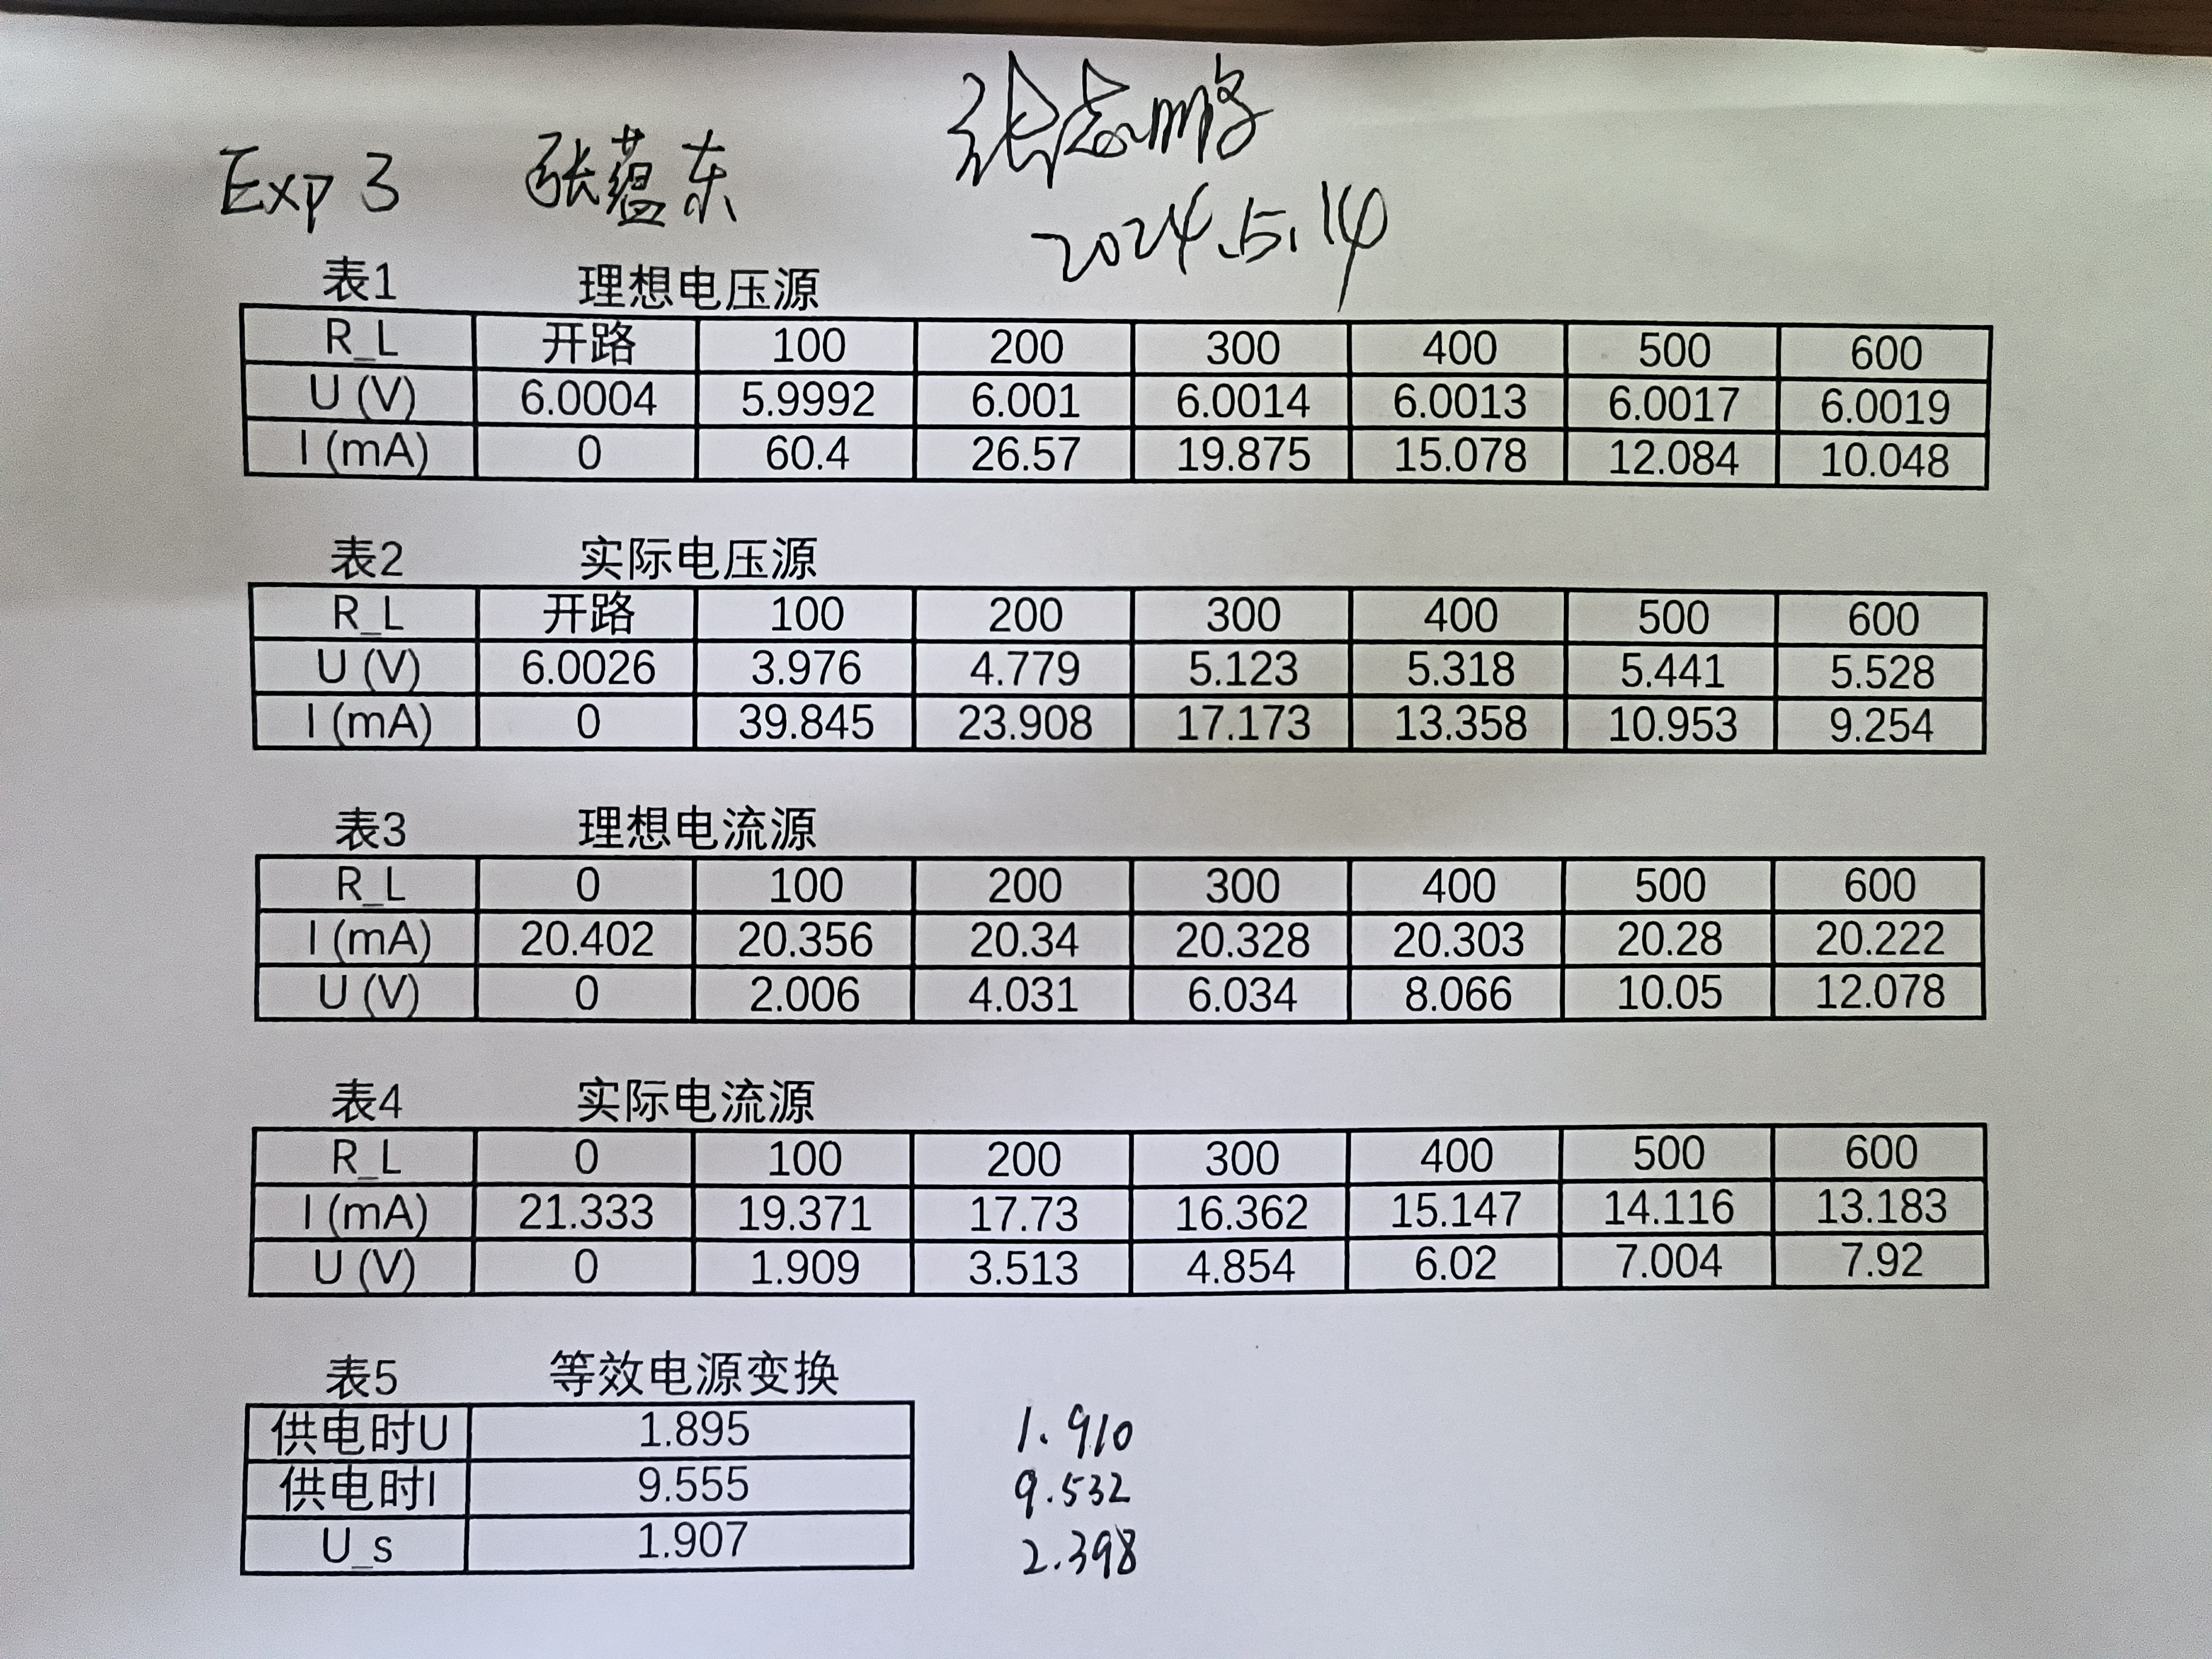
\includegraphics[width=0.95\textwidth]{data.jpg}}
    \end{center}

\end{document}